% !TEX TS-program = pdflatex
\documentclass[aspectratio=169]{beamer}
\usepackage[utf8]{inputenc}
\usepackage[T1]{fontenc}
\usetheme{Madrid}
\usecolortheme{seahorse}
\usefonttheme{professionalfonts}
\setbeamertemplate{navigation symbols}{}
\setbeamercovered{transparent}
\setbeamertemplate{itemize items}[circle]
\setbeamertemplate{enumerate items}[default]
\setlength{\parskip}{0.15em}

\definecolor{bepurple}{RGB}{107,63,160}
\definecolor{begold}{RGB}{200,168,75}
\definecolor{beteal}{RGB}{26,122,110}
\definecolor{berust}{RGB}{192,68,42}
\definecolor{beblue}{RGB}{26,74,138}
\definecolor{softpurple}{RGB}{240,232,255}
\definecolor{softgold}{RGB}{255,248,220}
\definecolor{softteal}{RGB}{220,242,240}
\definecolor{softrust}{RGB}{255,235,230}
\setbeamercolor{structure}{fg=beblue}
\setbeamercolor{title}{fg=white,bg=beblue}
\setbeamercolor{frametitle}{fg=beblue}
% Minimal block rendering: regular/example blocks become colored headings (no box)
\setbeamertemplate{block begin}{%
  \par\vspace{0.2ex}%
  \ifx\insertblocktitle\empty\else%
    {\usebeamerfont{block title}\color{beblue}\textbf{\insertblocktitle}}\par\vspace{0.2ex}%
  \fi%
}
\setbeamertemplate{block end}{\par\vspace{0.2ex}}
\setbeamertemplate{block example begin}{%
  \par\vspace{0.2ex}%
  \ifx\insertblocktitle\empty\else%
    {\usebeamerfont{block title}\color{beteal}\textbf{\insertblocktitle}}\par\vspace{0.2ex}%
  \fi%
}
\setbeamertemplate{block example end}{\par\vspace{0.2ex}}
\setbeamertemplate{block alerted begin}{%
  \par\vspace{0.5ex}%
  \begin{beamercolorbox}[sep=0.5ex,rounded=true,shadow=false]{block title alerted}%
    \usebeamerfont{block title}\insertblocktitle%
  \end{beamercolorbox}%
  \nointerlineskip%
  \begin{beamercolorbox}[sep=0.5ex,rounded=true,shadow=false]{block body alerted}%
    \usebeamerfont{block body}%
}
\setbeamertemplate{block alerted end}{\end{beamercolorbox}\par\vspace{0.5ex}}
\setbeamercolor{block title alerted}{fg=white,bg=berust}
\setbeamercolor{block body alerted}{fg=black,bg=berust!8}
\setbeamercolor{alerted text}{fg=berust}

\usepackage{booktabs,amsmath,amssymb,array,multirow,hyperref,colortbl,xcolor}
\usepackage{tikz}
\usepackage{pgfplots}
\pgfplotsset{compat=1.18}
\usetikzlibrary{arrows.meta,positioning,calc,shapes.geometric,patterns}
\hypersetup{colorlinks=true,linkcolor=beblue,urlcolor=beblue}

\title{\textbf{Lecture 5: Intertemporal Choice \& Savings Behaviour}}
\subtitle{Mental Accounting, Debt Traps, and the Retirement Crisis}
\author{Prof.\ Muhebullah Karimzada}
\institute{School of Economics, University of Northern British Columbia}
\date{ECON 230 $\cdot$ Introduction to Behavioural Economics $\cdot$ Winter 2027}

\begin{document}

\begin{frame}[plain]\titlepage\end{frame}

% ============================================================
\begin{frame}{Opening Puzzle --- Is Money Fungible?}
\note{Money IS fungible in standard economics --- a dollar is a dollar regardless of source. Mental accounting says NO. The responses to these three identical windfalls will differ. Poll the class.}
\begin{alertblock}{Poll --- Would You Spend These Differently?}
Scenario A: You won \textbf{\$5,000 in the lottery}.\\[0.3em]
Scenario B: You received a \textbf{\$5,000 tax refund from the CRA}.\\[0.3em]
Scenario C: Your employer gave you a \textbf{\$5,000 year-end bonus}.\\[0.4em]
\textbf{In each case: how much would you spend vs save?} Write down a number.
\end{alertblock}
\pause
\begin{block}{Standard Economics Says: Same Answer Every Time}
\$5,000 is \$5,000. Rational agents should save/spend the same fraction regardless of source. But research shows people \textit{systematically} treat these differently. Lottery winnings: spend. Tax refund: half-spend, half-save. Bonus: mostly save. This is \alert{mental accounting}.
\end{block}
\end{frame}

% ============================================================
\begin{frame}{Lecture Overview}
\begin{enumerate}[<+->]
  \item \textbf{Life Cycle Hypothesis} --- the standard model and its failures
  \item \textbf{Mental Accounting} --- money in separate ``buckets''
  \item \textbf{Sunk Cost Fallacy} --- past costs that should be ignored
  \item \textbf{The Debt Aversion Paradox} --- holding debt and savings simultaneously
  \item \textbf{The Canadian Savings Crisis} --- detailed data
  \item \textbf{Compound Interest Illusion} --- why people systematically underestimate growth
  \item \textbf{Behavioural Solutions} --- auto-enrollment, SMarT, simplification
  \item \textbf{The Credit Card Minimum Payment Trap} --- a numbers exercise
\end{enumerate}
\end{frame}

% ============================================================
\section{Life Cycle Hypothesis}
% ============================================================

\begin{frame}{The Life Cycle Hypothesis}
\textcolor{beblue}{\textbf{Modigliani \& Brumberg (1954):}} Rational agents maximise lifetime utility by \textbf{smoothing consumption}: borrow in \textbf{youth}, save in \textbf{prime years}, dissave in \textbf{retirement}.
\begin{columns}
\column{0.5\textwidth}
\begin{tikzpicture}
\begin{axis}[
  width=\textwidth,height=0.43\textheight,
  xlabel={\small Age},
  xmin=20,xmax=85,ymin=-55,ymax=120,
  axis lines=left,
  title={\small Life Cycle: Income, Consumption \& Net Savings},
  xtick={20,30,40,50,60,70,80},
  ytick={-50,0,50,100},
  yticklabels={$-50$,0,50,100},
  clip=false
]
\addplot[beteal,very thick,domain=20:80,samples=100]{100*sin(deg((x-20)*3.14159/60))*0.9+10};
\addplot[beblue,very thick,domain=20:80,samples=50]{55};
\addplot[berust,dashed,thick,domain=20:80,samples=100]{100*sin(deg((x-20)*3.14159/60))*0.9+10-55};
% Inline labels placed clearly outside overlap zones
\node[font=\tiny,beteal,right] at (axis cs:55,88) {Income};
\node[font=\tiny,beblue,right] at (axis cs:55,60) {Consumption};
\node[font=\tiny,berust,right] at (axis cs:55,28) {Net Savings};
\node[font=\tiny,berust,right] at (axis cs:21,-42) {\textit{Borrowing region}};
% Zero baseline
\draw[gray,thin,dashed] (axis cs:20,0) -- (axis cs:80,0);
\end{axis}
\end{tikzpicture}
\column{0.47\textwidth}
\begin{block}{Key Predictions}
\begin{enumerate}\small\setlength{\itemsep}{0pt}
  \item Temporary income shocks barely affect consumption.
  \item MPC from windfall $\approx 1/T$ (spread over remaining life).
  \item No response to predictable income changes.
  \item Dissave in retirement.
\end{enumerate}
\end{block}
\begin{alertblock}{All Four Fail}
\small Consumption is \textbf{too sensitive} to current income, \textbf{drops sharply} at retirement, and saving rates are far too low vs LCH predictions.
\end{alertblock}
\end{columns}
\end{frame}

% ============================================================
\begin{frame}{Excess Sensitivity --- Consumption Tracks Income}
\begin{block}{Flavin (1981); Carroll (2001)}
Consumption is too sensitive to current (predictable) income changes. If income is \textbf{fully predictable}, it should not change consumption (since it was already incorporated in the plan). But it does.
\end{block}
\begin{exampleblock}{Canadian Evidence}
\begin{itemize}
  \item Tax refunds: Canadians increase spending by \textbf{25--50\%} of refund in the refund month. Under LCH: should be $\approx 5\%$ (spread over 20-year horizon).
  \item Average Canadian tax refund (CRA, 2022): \$1,895.
  \item Retailers exploit this: ``Tax Refund Events'' in February--March. Canadian Tire, Walmart see \textbf{15--20\%} sales spikes in refund season.
  \item Souleles (1999): US consumption rises sharply when Social Security cheques arrive --- even though timing was 100\% predictable.
\end{itemize}
\end{exampleblock}
\end{frame}

% ============================================================
\section{Mental Accounting}
% ============================================================

\begin{frame}{Mental Accounting --- Thaler (1985, 1999)}
People \alert{categorise money into separate mental accounts} with different spending norms. \textcolor{beblue}{\textbf{The Three Accounts (Shefrin \& Thaler 1988):}}
\begin{columns}
\column{0.5\textwidth}
\begin{enumerate}\small
  \item \textbf{Current Income:} High MPC --- spend freely.
  \item \textbf{Current Assets:} Medium MPC --- savings, home equity.
  \item \textbf{Future Income:} Near-zero MPC --- RRSP. ``Don't touch.''
\end{enumerate}
\begin{alertblock}{The Paradox}
Households hold \textbf{credit card debt} at 19.99\% \textit{and} \textbf{RRSP} at 3\%. Should pay off the card --- but mental accounts prevent this.
\end{alertblock}
\column{0.47\textwidth}
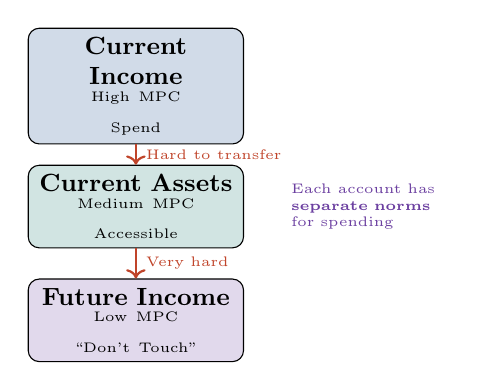
\begin{tikzpicture}[scale=0.85]
\node[draw,fill=beblue!20,rounded corners,text width=2.5cm,align=center,font=\small] (ci) at (0,3) {\textbf{Current Income}\\\tiny High MPC\\\tiny Spend};
\node[draw,fill=beteal!20,rounded corners,text width=2.5cm,align=center,font=\small] (ca) at (0,1.2) {\textbf{Current Assets}\\\tiny Medium MPC\\\tiny Accessible};
\node[draw,fill=bepurple!20,rounded corners,text width=2.5cm,align=center,font=\small] (fi) at (0,-0.5) {\textbf{Future Income}\\\tiny Low MPC\\\tiny ``Don't Touch''};
\draw[->,thick,berust] (ci) -- node[right,font=\tiny,berust]{Hard to transfer} (ca);
\draw[->,thick,berust] (ca) -- node[right,font=\tiny,berust]{Very hard} (fi);
\node[font=\tiny,bepurple,text width=2cm] at (3.5,1.2) {Each account has\\\textbf{separate norms}\\ for spending};
\end{tikzpicture}
\end{columns}
\end{frame}

% ============================================================
\begin{frame}{The Sunk Cost Fallacy}
Past costs that are \textbf{irretrievable} should not affect current decisions. Only future costs and benefits matter.
\begin{columns}
\column{0.5\textwidth}
\begin{alertblock}{The Theatre Ticket}
\$50 ticket; snowing; feel sick. Go?\\[0.2em]
\textbf{If PAID:} Most say yes (don't ``waste'' it).\\
\textbf{If FREE:} Most say no.\\[0.2em]
But \$50 is \alert{gone either way}. Only relevant question: is going worth the discomfort?
\end{alertblock}
\column{0.47\textwidth}
\begin{exampleblock}{Real Examples}
\begin{itemize}\small
  \item Bad relationship ``after all the time invested.''
  \item Holding a losing stock ``because I can't sell at a loss.''
  \item Finishing a terrible movie ``because we paid.''
  \item The Concorde: continued for sunk development costs.
\end{itemize}
\end{exampleblock}
\end{columns}
\end{frame}

% ============================================================
\begin{frame}{[GAME] The Ski Trip Sunk Cost}
\note{This is a classic sunk cost experiment. The key manipulation is whether the ticket was paid or received free. Typically 80\%+ say YES in scenario A, 30\% in scenario B. The difference reveals the sunk cost effect.}
\begin{alertblock}{Scenario A --- Left Side of Room}
\small One month ago, you bought a \textbf{non-refundable} ski lift ticket for \$80. Today, the day of the trip, you feel mildly sick and hear snow conditions are icy and dangerous.\\[0.2em]
\textbf{Do you go skiing?} Yes / No
\end{alertblock}
\begin{alertblock}{Scenario B --- Right Side of Room}
\small One month ago, a friend gave you a \textbf{free} ski lift ticket (worth \$80). Same day: you feel mildly sick, conditions are icy.\\[0.2em]
\textbf{Do you go skiing?} Yes / No
\end{alertblock}
\pause
\begin{block}{Expected Results \& Discussion}
\small Far more students say YES in Scenario A. But the \$80 is gone either way. The only relevant question is: \textit{Is skiing today worth the discomfort and risk?} If not in B, it should not be in A. The difference is the \alert{sunk cost fallacy}.
\end{block}
\end{frame}

% ============================================================
\begin{frame}{The Debt Aversion Paradox}
Average Canadian household: \textbf{credit card debt} \$4,200 at 19.99\% APR \textit{and} \textbf{TFSA} \$18,000 at 3--4\%.

\textbf{The arbitrage:} Pay off the card with TFSA savings = \textbf{guaranteed 17\% risk-free return}. Obvious --- but mental accounts prevent it.
\begin{columns}
\column{0.5\textwidth}
\begin{exampleblock}{Gross, Souleles (2002)}
US households: \$5K liquid assets + \$5K credit card debt at 18\%. Should pay down. \textbf{Only 12\%} do. ``Emergency fund'' and ``credit card'' are separate mental accounts.
\end{exampleblock}
\column{0.47\textwidth}
\begin{block}{Behavioural Explanation}
\begin{itemize}\small
  \item TFSA = ``emergency fund'' (don't touch)
  \item Credit card = ``current spending''
  \item Transferring violates mental account norms
  \item Loss aversion: dipping in feels like a loss
\end{itemize}
\end{block}
\end{columns}
\end{frame}

% ============================================================
\section{The Compound Interest Illusion}
% ============================================================

\begin{frame}{Compound Interest Is Always Underestimated}
\begin{block}{Wagenaar \& Sagaria (1975)}
People systematically \textbf{underestimate compound growth}. They apply a \textit{linear} mental model to what is an exponential process.
\end{block}
\begin{columns}
\column{0.5\textwidth}
\begin{tikzpicture}
\begin{axis}[
  width=\textwidth,height=0.52\textheight,
  xlabel={\small Years},ylabel={\small Value (\$)},
  xmin=0,xmax=40,ymin=0,ymax=16000,
  axis lines=left,
  title={\small \$1{,}000 Invested at 7\%/year},
  legend pos=north west
]
\addplot[black,dashed,domain=0:40,samples=40]{1000+70*x};
\addplot[beteal,very thick,domain=0:40,samples=100]{1000*exp(0.0677*x)};
\addplot[berust,thick,domain=0:40,samples=100]{1000*exp(0.0953*x)};
\node[font=\tiny,black] at (axis cs:35,3300) {Linear (wrong)};
\legend{\small Linear guess,\small 7\% compound,\small 10\% compound}
\end{axis}
\end{tikzpicture}
\column{0.47\textwidth}
\begin{alertblock}{The Numbers}
\small\$1,000 at 7\% annual return:
\begin{itemize}\setlength{\itemsep}{0pt}
  \item After 10 years: \textbf{\$1,967}
  \item After 20 years: \textbf{\$3,870}
  \item After 30 years: \textbf{\$7,612}
  \item After 40 years: \textbf{\$14,974}
\end{itemize}
\textit{Student guess for 40 years: \$3,800.} Underestimate by \textbf{75\%}. The ``Rule of 72'': money doubles every $72/r$ years.
\end{alertblock}
\end{columns}
\end{frame}

% ============================================================
\begin{frame}{The Minimum Payment Trap}
\textbf{\$5,000} at \textbf{19.99\% APR}. Minimum payment = 2\% of balance.
\begin{columns}
\column{0.5\textwidth}
\begin{tikzpicture}
\begin{axis}[
  width=\textwidth,height=0.58\textheight,
  xlabel={\small Years},ylabel={\small Balance (\$)},
  xmin=0,xmax=40,ymin=0,ymax=5500,
  axis lines=left,
  title={\small Debt Repayment: \$5{,}000 at 19.99\%},
  legend pos=north east
]
\addplot[berust,very thick] coordinates{(0,5000)(5,4500)(10,3800)(20,2700)(30,1500)(37,100)(37.5,0)};
\addplot[beteal,very thick] coordinates{(0,5000)(1,3200)(2,1400)(2.5,0)};
\legend{\small Min payment (37 yrs),\small \$200/mo fixed (2.5 yrs)}
\end{axis}
\end{tikzpicture}
\column{0.47\textwidth}
\begin{alertblock}{Min Payment: 37 yrs, \$10K+ interest}
Pays off in \textbf{37 years}; total interest \textbf{\$10,233} --- more than double the debt.
\end{alertblock}
\textcolor{beteal}{\textbf{\$200/mo:}} Pays off in \textbf{2.5 years}; interest \textbf{\$1,065}; saves \textbf{\$9,168}.

\textcolor{bepurple}{\textbf{FCAC (2021):}} Statements must now disclose payoff time and total interest $\Rightarrow$ higher payments up 12\%.
\end{columns}
\end{frame}

% ============================================================
\begin{frame}{Auto-Enrollment --- The Power of Defaults}
\textcolor{beblue}{\textbf{Madrian \& Shea (2001):}} One US company changed 401(k) from \textbf{opt-in} to \textbf{opt-out}. Same plan, same rates --- different default.
\begin{columns}
\column{0.5\textwidth}
\begin{tikzpicture}
\begin{axis}[
  width=\textwidth,height=0.52\textheight,
  xlabel={\small Months at Company},ylabel={\small Participation (\%)},
  xmin=0,xmax=36,ymin=0,ymax=100,
  axis lines=left,
  title={\small Opt-In vs Opt-Out (Madrian \& Shea 2001)},
  legend pos=south east
]
\addplot[beteal,very thick] coordinates{(0,86)(6,88)(12,89)(24,91)(36,93)};
\addplot[berust,very thick] coordinates{(0,10)(6,25)(12,35)(24,43)(36,49)};
\legend{\small Opt-Out (default = enroll),\small Opt-In (must choose)}
\end{axis}
\end{tikzpicture}
\column{0.47\textwidth}
\begin{block}{Same Plan. Different Default. Massive Difference.}
\begin{itemize}
  \item Opt-in: \textbf{49\%} enrolled after 3 years.
  \item Opt-out: \textbf{86\%} enrolled immediately; \textbf{93\%} after 3 years.
  \item Mechanism: inertia + implicit endorsement.
\end{itemize}
\end{block}
\textcolor{beteal}{\textbf{Canada:}} Australia Superannuation = 11\% mandatory (ultimate default). PRPP opt-in = low uptake. Federal pilot (2019): participation $+$40\%.
\end{columns}
\end{frame}

% ============================================================
\begin{frame}{Financial Literacy in Canada}
\textcolor{beblue}{\textbf{Lusardi \& Mitchell (2011) --- The Big Three:}}
\begin{enumerate}\small
  \item \textbf{Compound interest} (\$100@2\%, 5 yrs: more than \$110?): \textcolor{beteal}{67\%} correct.
  \item \textbf{Inflation} (1\% savings, 2\% inflation: buy more/less?): \textcolor{beteal}{75\%} correct.
  \item \textbf{Diversification} (one stock safer than mutual fund?): \textcolor{berust}{52\%} correct.
\end{enumerate}
\begin{alertblock}{Canadian Data}
\begin{itemize}\small
  \item All three correct: only \textbf{42\%} of Canadians.
  \item Correct answers predict \textbf{10$\times$ larger retirement savings}.
  \item \textbf{BUT} financial education programs: only $+0.1\%$ savings rate improvement (Fernandes et al., 2014). Information alone is insufficient.
\end{itemize}
\end{alertblock}
\end{frame}

% ============================================================
\begin{frame}{Discussion Questions}
\begin{enumerate}
  \item[\textcolor{bepurple}{Q1.}] ``Do you have a personal emergency fund? Is it in a separate account from your chequing account? Does mental accounting help you or hurt you here?''
  \medskip
  \item[\textcolor{beteal}{Q2.}] ``Should Canada move to a mandatory defined-contribution pension system like Australia's Superannuation (11\% of every paycheque)? What are the trade-offs?''
  \medskip
  \item[\textcolor{berust}{Q3.}] ``Banks are required to display minimum-payment consequences on credit card statements. Is this enough? What else could be done?''
\end{enumerate}
\end{frame}

% ============================================================
\begin{frame}{Key Takeaways --- Lecture 5}
\begin{itemize}\small\setlength{\itemsep}{0pt}
  \item[\textcolor{beteal}{\checkmark}] \textbf{LCH predicts consumption smoothing} --- evidence shows excess sensitivity and undersaving.
  \item[\textcolor{beteal}{\checkmark}] \textbf{Mental accounting:} money is NOT fungible across mental accounts; each account has different spending norms.
  \item[\textcolor{beteal}{\checkmark}] \textbf{Sunk cost fallacy:} past costs affect current decisions even when they shouldn't.
  \item[\textcolor{beteal}{\checkmark}] \textbf{Debt aversion paradox:} hold debt and savings simultaneously because they are in separate mental accounts.
  \item[\textcolor{beteal}{\checkmark}] \textbf{Compound interest illusion:} people apply linear thinking to exponential processes --- systematically underestimating savings growth.
  \item[\textcolor{beteal}{\checkmark}] \textbf{Solutions:} auto-enrollment defaults, SMarT escalation, simplification, salience of long-run costs.
  \item[\textcolor{beteal}{\checkmark}] \textbf{Canadian context:} RRSP gap, TFSA underutilization, credit card debt at record high, savings rate at historic low.
\end{itemize}
\smallskip\textcolor{beblue}{\textbf{Next:}} \textbf{Lecture 6: Social Preferences} --- We move from individual decisions to strategic interactions. Why do people give money away, reject unfair offers, and punish free-riders at personal cost?
\end{frame}

\end{document}
